\section{Подсистема имитационного моделирования}
\indent Подсистема имитационного моделирования - модуль, производящий моделирование производственных процессов для для получения приблизительной оценки времени выполнения набора операций (например карты технологического процесса).\\
\indent Карта технологического процесса - документ, предназначенный для операционного описания технологического процесса изготовления или ремонта изделия (составных частей изделия) в технологической последовательности по всем операциям одного вида формообразования, обработки, сборки или ремонта с указанием переходов, технологических режимов и данных о средствах технологического оснащения, материальных и трудовых затратах.\\

\begin{figure}[h]
	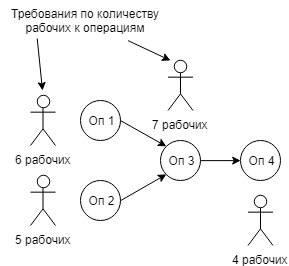
\includegraphics[width=\linewidth]{pics/techMapViz.png}
	\caption{Визуальное представление технологической карты с ограничением по количеству рабочих на операцию}
	\label{fig:map}
	\centering
\end{figure}

\indent Для определения оценки времени модуль рассматривает карту технологического процесса как систему уравнений, в которой неизвестными являются времена начала выполнения операций.
Каждое уравнение предстает в виде $x_n = x_{n-1} + dur$, а система в целом:
\todo{система уравнений}
\begin{equation}
	x_n = x_{n-1} + dur
\end{equation}

\indent В начале работы система выберет одно из уравнений (в зависимости от накладываемых моделью ресурса, о которой пойдет речь в следующем разделе, ограничений), которое может быть рассчитано, то есть которое может начинаться с логического нуля и произведет подсчет времени, когда закончится выполнение данной операции.
Затем по тому же принципу будет выбрано следующее уравнение и так далее пока есть неразрешенные переменные.
Когда они закончатся система завершит свое выполнение, передав результирующее значение и необходимые данные другому модулю, который произведет отображение полученного подсистемой имитационного моделирования числа в физическое, о чем речь пойдет ниже.

\todo[inline]{система уравнений}
\todo[inline]{схема и описание}
